The code used to check whether the test will determine the sequence as convergent or divergent. At the bottom is a plotted graph of the sequence made in 3a.
\begin{verbatim}
xs = np.linspace(-5, 5, 101)
ys = np.zeros(xs.shape)

epsilon = 1

for i in range(101):
    #put the function to be tested here
    if i < 50:
        ys[i] = 1/(i+1) #1/n
    else:
        ys[i] = ys[i-1] + 1/(i+1)
    
    
    
    
isconvergent = True
    
for i in range(ys.size):
    if i > 1:
        if abs(ys[i-1]-ys[i]) > epsilon and isconvergent:
            isconvergent = False
            print ("is not convergent")
            
if isconvergent:
    print ("is convergent")
    
# Removing lines drawn where the function is discontinuous
pos = np.where(np.abs(np.diff(ys)) >= 1)[0]+1
xs = np.insert(xs, pos, np.nan)
ys = np.insert(ys, pos, np.nan)
    
plt.plot(xs, ys) # Plotting 
plt.title('Exercise 3.b')
plt.xlabel('x')
plt.ylabel('y')
\end{verbatim}
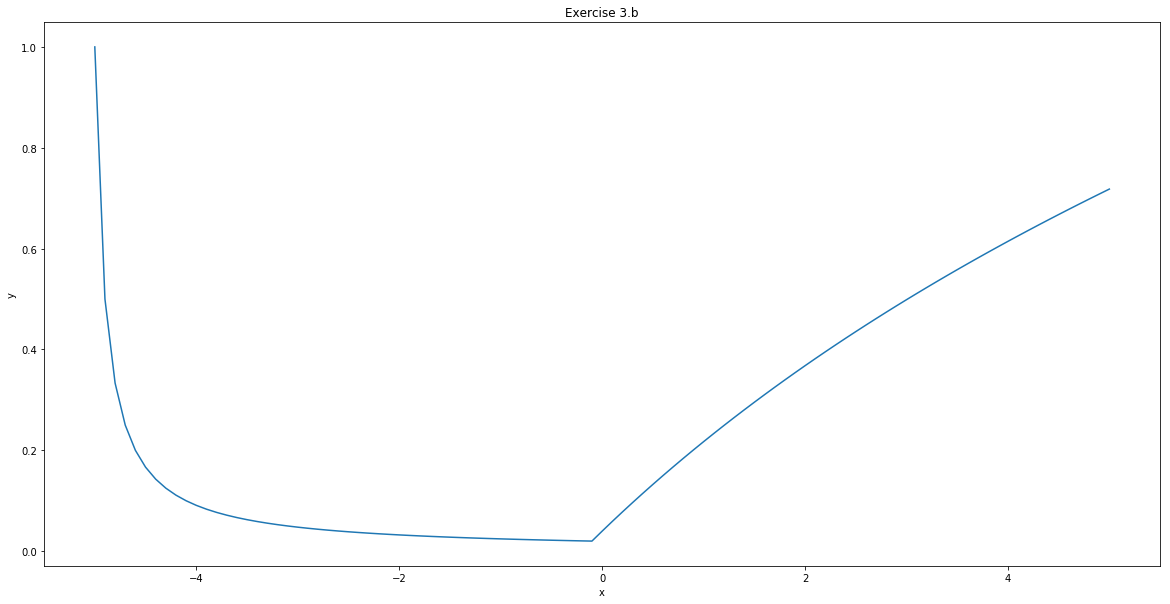
\includegraphics[width=\linewidth]{3bgraph.png}